Apparatur\section{Theorie}
Der Germaniumdetektor wird zur $\gamma$-Spektroskopie verwendet, da dieser
gegenüber eines Szintillations-Detektors eine viel höhere Auflösung besitzt.
(Szintillationsdetektor: $\approx \SI{13}{\kilo\eV} $,
Germaniumdetektor:$\approx \SI{895}{\eV} $ bei $E_{\gamma}=\SI{500}{\kilo\eV}$
\cite{Q1})

\subsection{Wechselwirkung von Gamma-Strahlung mit Materie}
In Abbildung \ref{abb:1} sind die Extinktionskoeffizienten der verschiedenen
Wechselwirkungen mit Materie zu erkennen.
Es wurde dabei der Extinktionskoeffizient, ein Maß für den Energieverlust,
gegen die Energie der $\gamma$-Quanten aufgetragen.
Zur Beschreibung der Wechselwirkungen, ist es notwendig auch den Wirkungsquerschnitt
zu betrachten. Dieser beschreibt die Wahrscheinlichkeit der Wechselwirkung mit
der Materie. Diese hängt von der Energie der $\gamma$-Quanten und der
Eigenschaften des Materials ab. Die verschiedenen Wechselwirkungen werden im
Folgenden näher erklärt.

Bei dem Photoeffekt gibt das $\gamma$-Quant die komplette Energie
an ein Hüllenelektron (meist aus der K-Schale) eines Atoms ab. Übersteigt die
Energie des $\gamma$-Quants
die Bindungsenergie des Elektrons, so wird dieses aus dem Atom
herausgelöst. Die übrige Energie erhält das Elektron als kinetische Energie.
Da bei dem Herauslösen des Elektrons ein Loch entsteht, wird dieses durch ein
anderes Elektron einer höheren Schale aufgefüllt. Dabei wird Energie in Form
von $\gamma$-Strahlung frei, welche ein weiteres Elektron aus einer höheren
Schale herauslösen kann. Dieses zweite herausgelöste Elektron wird Auger-Elektron
genannt.
Der Wirkungsquerschnitt $\sigma_{\symup{Ph}}$ für den Photoeffekt ist stark
abhängig von der Energie  $E$ der $\gamma$-Quanten und der Kernladungszahl $Z$ des
Materials:
\begin{equation}
  \sigma_{\symup{Ph}} \propto Z^{\alpha}E^{\delta} \, ,
\end{equation}
wobei die Exponenten empirisch festgestellt wurden ($4<\alpha<5$ und
$\delta \approx -3,5$). Für Energien ab \SI{5}{\mega\eV} kann $\delta$ auf
einen Wert bis zu -1 steigen.

Eine weitere wichtige Wechselwirkung ist der Compton-Effekt.
Hierbei streut das $\gamma$-Quant elastisch an einem quasi freien Elektron und gibt
einen Teil seiner Energie an dieses in Form von kinetischer Energie ab.
Die Streuung bewirkt eine Energieabnahme und Richtungsänderung des
$\gamma$-Quants, wobei ein maximaler Energieübertrag bei einer Richtungsänderung
von $\Psi_{\gamma} = \pi$ stattfindet:
\begin{equation}
  E_{\gamma}' = E_{\gamma} \cdot ( 1+\epsilon(1-\cos{\Psi_{\gamma}}))^{-1} \;
  \symup{mit} \; \epsilon = \frac{E_{\gamma}}{m_0c²}
\end{equation}
Die Herleitung des Wirkungsquerschnitts $\sigma_{\symup{Co}}$ für den Compton-Effekt
ist sehr lang und kompliziert und wird hier nicht weiter erläutert.
Aus dieser Herleitung folgt:
\begin{equation}
  \label{eq:WQ}
  \sigma_{\symup{Co}}=\frac{3}{4}\sigma_{\symup{Th}}
  \left( \frac{1+\epsilon}{\epsilon^2} \left[ \frac{2+2\epsilon}{1+2\epsilon} -
  \frac{1}{\epsilon} \ln{(1+2\epsilon)} \right] +
  \frac{1}{2\epsilon}\ln{(1+2\epsilon)} -
  \frac{1+3\epsilon}{(1-2\epsilon)^2}\right)
\end{equation}
mit
\begin{equation}
  \sigma_{\symup{Th}} = \frac{8}{3}\pi \left(\frac{e_0}{4 \pi \epsilon_0 c^2 m_o} \right)^2
  := \frac{8}{3}\pi r_e^2
\end{equation}
wobei $e_o$ die Elementarladung, $c$ die Vakuumlichtgeschwindigkeit,
$\epsilon_0$ die Influenzkonstante, $m_0$ die Masse eines Elektrons und
$r_e$ den klassischen Elektronenradius darstellt.

Bei der Paarerzeugung wird ein Elektron und ein Positron erzeugt.
Hierbei muss ein $\gamma$-Quant aufgrund der Impulserhaltung an einem Potential
eines Atomkerns oder eines Elektrons gestreut werden, um ein Elektron und ein
Positron erzeugen zu können.
Bei einem Atom als Stoßpartner muss die Energie des $\gamma$-Quants
mindestens gleich der Ruheenergie von einem Elektron und einem Positron sein,
da hierbei die Energie in Masse umgewandelt wird. Der Impuls wird hierbei
an das Atom weitergegeben. Bei einem Elektron als Stoßpartner muss das
$\gamma$-Quant mindestens die vierfache Ruheenergie eines Elektrons besitzen,
da hier der Impuls nicht komplett an das Stoßelektron übergeben werden kann,
aufgrund der geringen Masse des Elektrons.
Der Wirkungsquerschnitt $\sigma_{\symup{Pa}}$ der Paarerzeugung kann mit viel
Aufwand hergeleitet werden. Hier sind zwei exemplarische Ergebnisse dargestellt,
wobei unterschieden werden muss für kernnahe und kernferne Paarbildung.
Für die kernnahe Paarbildung, also Bereiche von (10-25)\,\si{\mega\eV}, gilt
die folgende Gleichung:
\begin{equation}
   \sigma_{\symup{Pa}}= \alpha r_e^2Z^2 \left( \frac{28}{9} \ln{(2 \epsilon)} -
   \frac{218}{27} \right)
\end{equation}
Für die kernferne Paarbildung (außerhalb der Elektronenhülle) lässt sich der
Wirkungsquerschnitt wie folgt berechnen:
\begin{equation}
  \sigma_{\symup{Pa}}= \alpha r_e^2Z^2 \left( \frac{28}{9} \ln{\left(\frac{183}{\sqrt[3]{Z}}\right)} -
  \frac{2}{27} \right)
\end{equation}
Diese Gleichung gilt für Energien, die größer sind als \SI{500}{\mega\eV}.


\begin{figure}
  \centering
  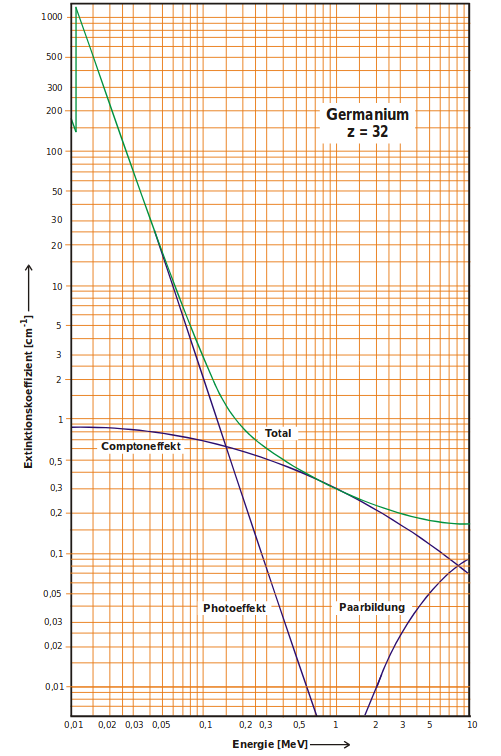
\includegraphics[scale=0.8]{Wechselwirkungen.png}
  \caption{Die Extinktionskoeffizienten der verschiedenen Wechselwirkungen von $\gamma$-Quanten mit Germanium. \cite{Q1}}
  \label{abb:1}
\end{figure}

\subsection{Aufbau und Wirkungsweise eines Germaniumdetektors}
Der Halbleiter-Detektor besteht im Wesentlichen aus einer Halbleiterdiode,
welche aus zwei Schichten besteht: Der n-dotierten Schicht als
Elektronen-Donator und einer p-dortierten Schicht als Elektronen-Akzeptor.
In dem Bereich zwischen den beiden Schichten entsteht eine Sperrschicht. Durch
Rekombination der Löcher aus der p-Schicht und der Elektronen aus der n-Schicht,
entsteht hier eine Zone ohne freie Ladungsträger.
Die benannten Löcher sind Elektronenlöcher, welche hier wie positiv geladene
Teilchen angesehen werden können. Diese entstehen zum Beispiel durch p-Dotierung von Germanium
(4 Valenzelektronen) mit Bohr, welche nur 3 Valenzelektronen besitzt. Dadurch
entsteht durch die Einbindung von Bohr in das Gitter des Germaniums ein
Elektronenloch, bzw. eine nicht besetzte Elektronenstelle.
Die Sperrschicht ist wichtig für die Funktionsweise eines Germaniumdetektors,
da hier die Wechselwirkung zwischen den $\gamma$-Quanten und der Materie
stattfindet, bzw. nur hier die Wechselwirkung zu einem Zählereignis führt.
In der Sperrschicht werden Elektronen durch die vorher benannten Wechselwirkungen
mit sehr hohen kinetischen Energien freigesetzt. Diese widerum regen andere
Elektronen an, die zwar geringere kinetische Energien haben, aber genug, um die
Lücke zwischen dem Leitungsband und dem Valenzband zu überspringen. So
entstehen in der Sperrschicht bzw. ladungsträgerarmen Zone Löcher und Elektronen,
die durch eine außen anliegende Spannung getrennt werden können, ohne wieder zu
rekombinieren. Durch diesen Vorgang entsteht ein Stromfluss, welcher zu einem
Zählereignis führt.
Um ein möglichst genaues Messergebnis zu erhalten, ist es sinnvoll, die
ladungsträgerarme Zone zu verbreitern, denn die Breite beträgt ohne äußere Einflüsse
nur einige \si{\micro\meter}. Eine hohe außen angelegte Spannung (einige \si{\kilo\volt}) vergrößert
die ladungsträgerarme Zone auf einige \si{\centi\meter}.
Dies ist nur begrenzt möglich, da die Hochspannung dazu führt, dass die
freigesetzen thermischen Elektronen auch zu den verschiedenen Elektroden
beschleunigt werden. Somit wird Strom erzeugt, der die Messergebnisse
verfälscht. Deswegen wird während der Messung der Germaniumkristall mit
flüssigem Stickstoff auf $\SI{77}{\kelvin}$ gekühlt.
Außerdem ist die Dicke $d$ der Sperrschicht abhängig von der Dotierung
der Schichten, wie in Gleichung \eqref{eq:1} zu sehen.

\begin{equation}
  \label{eq:1}
  d = d_p + d_n \approx d_p \approx \sqrt{\frac{2 \epsilon \epsilon_0}
  {e_0}(U_D+U) \frac{1}{n_A}},
\end{equation}
wobei $d_p$ die Breite der Sperrschicht in der p-dotierten Schicht, $d_n$
die Breite der Sperrschicht in der n-dotierten Schicht, $U$ die angelegte
Sperrspannung und $U_D$ das Diffusionspotential beschreibt.
Um die Dicke also zu vergrößern ist es sinnvoll, die Akzeptorendichte $n_A$ so
gering wie möglich zu halten. Deswegen wird für einen Germaniumdetektor ein
sehr reiner Germanium-Kristall mit $n_A \approx 10^{10}\,
\frac{\symup{Atome}}{\symup{cm}} $ verwendet.

Der schematische Aufbau eines Germaniumdetektors ist in Abbildung \ref{abb:3}
zu sehen.

\begin{figure}
  \centering
  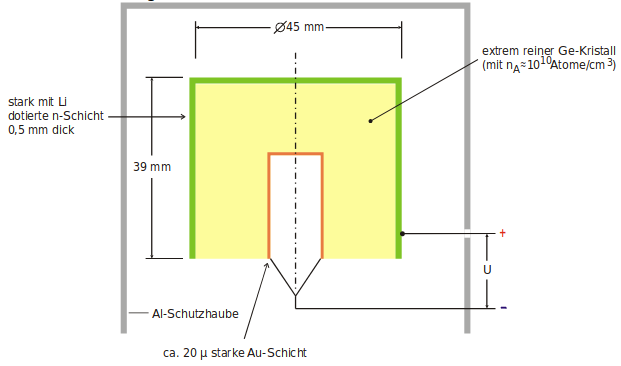
\includegraphics[scale=0.5]{AufbauDetektor.png}
  \caption{Schematischer Aufbau eines Germaniumdetektors. \cite{Q1}}
  \label{abb:3}
\end{figure}

Als p-dotierte Schicht und zusätzlich als Anschluss für die Hochspannung wird
eine dünne Schicht aus Gold auf die Innenseite des Germaniumskristalls aufgedampft.
Als n-dotierte Schicht ist der Germaniumkristall auf der Außenseite von einer
Lithiumschicht umgeben. Der Detektor ist außerdem mit einer Aluminium
Schutzhaube umgeben für eine thermische Isolation. Zusätzlich wird die natürliche
Untergrundstrahlung durch eine Blei-Schicht abgeschirmt, um die Messergebnisse
nicht zu verfälschen.
Um gegebenenfalls strahlende Isotope aus dem Blei abzuschirmen, wird noch eine
weitere Schicht aus Kupfer unter der Blei-Schicht angebracht.

\subsection{Energiespektrum}
In Abbildung \ref{abb:4} ist das Energiespektrum eines monochromatischen
$\gamma$-Strahlers zu sehen. Der Photopeak ensteht durch vollständige Abgabe der Enerige
durch den Photoeffekt.
Das Compton-Kontinuum wird durch die Comptonstreuung hervorgerufen.
Hierbei wird nur ein Teil der Energie abgegeben, deswegen ist dies für die
Energiebestimmung des $\gamma$-Quants nicht nützlich. Die Comptonkante entsteht durch
den maximalen Energieübertrag bei einer Richtungsänderung des $\gamma$-Quants von $\pi$.
Nach der Compton-Kante ist dennoch eine Intensität zu erkennen. Diese kommt
durch mehrfach compton-gestreute $\gamma$-Quants zustande.
Der Rückstreupeak ensteht auch durch Comptonstreuung, aber
nicht in dem Detektor, sondern in der Umgebung, beispielsweise in der
Abschirmung.

\begin{figure}
  \centering
  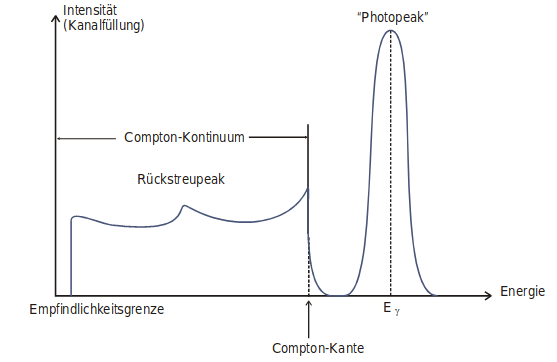
\includegraphics[scale=0.5]{Spektrum.png}
  \caption{Spektrum eines monochromatischen $\gamma$-Strahlers. \cite{Q1}}
  \label{abb:4}
\end{figure}

\subsection{Energetisches Auflösungsvermögen und Effizienz}

Eine Kenngröße für das energetische Auflösungsvermögen ist die Halbwertsbreite
$\Delta E_{1/2}$ der Impulsverteilung bei monochromatischer $\gamma$-Strahlung,
denn Spektrallinien mit einem Energieunterschied von $\Delta E_{1/2}$
können noch gut voneinander unterschieden werden.
Die Halbwertsbreite wird durch die Anzahl der erzeugten
Elektronen-Loch-Paare durch ein $\gamma$-Quant festgelegt.
Außerdem werden bei der Erzeugung von einem Elektronen-Loch-Paar zusätzlich
Phononen erzeugt. Das kann aus der Differenz der Bildungsenergie des
Elektronen-Loch-Paars (hier etwa \SI{2,90}{\eV}) und der Energielücke zwischen
dem Leitungs- und Valenzband (hier etwa \SI{0,67}{\eV}) gefolgert werden, da
diese Energiedifferenz statistisch auf das Elektronen-Loch-Paar und die Phononen
verteilt wird.

Da die Ladungsträgerverteilung nicht komplett unkorreliert verläuft, sondern
die Fluktuation der Ladungsträgererzeugung durch die Fluktuation der
Phononenanregung kompensiert wird, wird der Fano-Faktor $F$ eingeführt ($F<1$).
Bei diesem Versuch liegt der Fano-Faktor bei etwa $F=0,1$.
Damit folgt für die Standardabweichung $\sigma$
\begin{equation}
  \sigma = \sqrt{F\overline{n}} = \sqrt{F \frac{E_{\gamma}}{E_{\symup{El}}}}
\end{equation}
(Fano-Faktor $F$, Energie der $\gamma$-Quanten $E_{\gamma}$, Bildungsenergie der
Elektronen-Loch-Paare $ E_{\symup{El}}$).
Da die Anzahl der erzeugten Elektronen-Loch-Paare $n>>1$ ist, kann die
Poissonverteilung mit einer Gaußverteilung angenähert werden:
\begin{equation}
  \Delta E_{1/2} = \sqrt{2\ln{(2)}}\sigma_E =\sqrt{8\ln{(2)}}\frac{\sigma}{\overline{n}}
  E_{\gamma} = 2,35\sqrt{0,1E_{\gamma}E_{\symup{El}}}
\end{equation}
Die Halbwertsbreite des Germaniumdetektors bei einer typischen Energie von
\SI{500}{\kilo\eV} liegt bei:
\begin{align}
    \label{eq:halbwertsbreite}
    \Delta E_{1/2}(\SI{500}{\kilo\eV})= 2,35 \sqrt{0,1 \cdot 500000\cdot 2,9} \approx \SI{895}{\eV} \; .
\end{align}


Durch einige Einflüsse wird das energetische Auflösungsvermögen vermindert:
\begin{itemize}
  \item Rauschen des Leckstroms, durch Eigenleitung und Restverunreinigung.
  Dies wird durch Abkühlen der Apparatur verringert.
  \item Rauschen des Verstärkers
  \item unvollständige Ladungssammlung durch Feldinhomogenitäten
\end{itemize}
Diese Störeinflüsse addieren sich unkorreliert zur theoretischen Halbwertsbreite
dazu.

Die Effizienz bezeichnet die Energieabhängigkeit der Nachweiswahrscheinlichkeit
bei der Detektion von $\gamma$-Quanten.
Die Effizienz Q eines Germaniumdetektors kann mit Hilfe einiger Parameter berechnet werden:
\begin{equation}
    \label{eq:effizienz}
    \text{Q} = \frac{4 \pi \text{Z}}{\Omega \text{A} \Delta \text{t} \text{W}}
\end{equation}
Hierbei beschreibt A die Aktivität der Probe am Versuchstag, W die Emissionswahrscheinlichkeit, Z das gemessene Zählergebnis als Summe der Impulse in einem Peak, $\delta t$ den Messzeitraum und $\Omega$ den Raumwinkel.
Das Raumwinkelelement $\frac{\Omega}{4\pi}$ berechnet sich wie folgt:
\begin{equation}
    \label{eq:Omega}
    \frac{\Omega}{4 \pi} = \frac{1}{2} \left(1- \frac{a}{\sqrt{a^2 + r^2}} \right)
\end{equation}

\begin{figure}
  \centering
  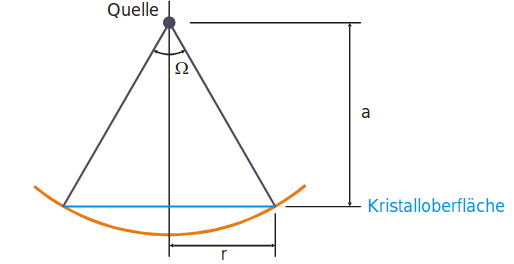
\includegraphics[scale=0.7]{Raumwinkel.png}
  \caption{Geometische Veranschaulichung zur Berechnung des Raumwinkels. \cite{Q1}}
  \label{abb:Raumwinkel}
\end{figure}

\subsection{Aufbau}

Der Blockschaltbild des Versuchs ist in Abbildung \ref{abb:2} zu sehen. Folgende
Komponenten sind in dem Aufbau enthalten: Detektor, Vorverstärker, Hauptverstärker,
Vielkanalanalysator, Temperaturregler.

Der Detektor dient zur Detektion der $\gamma$-Quanten mit Hilfe
einer Halbleiterdiode.

Der Vorverstärker integriert den vom Detektor
kommenden Strom in einen Spannungsimpuls, da Spannung mit geringeren
Verlusten weitergeleitet werden kann als Strom. Damit die eintreffenden Signale
nicht nacheinander aufaddiert werden und somit keine Aussage über die Höhe der
einzelnen Signale mehr getroffen werden kann, muss der Kondensator nach jedem
Ladungsimpuls entladen werden. Da durch eine
Entladung über einen Widerstand ein Rauschen entsteht, wird der Kondensator
durch eine optoelektronische Rückkopplung entladen, bei der die
Gate-Drain-Schicht der Feldeffekttransistoren
des Operationsverstärkers mit einer LED beleuchtet wird, wobei die
Sperrschicht kurz leitend wird und die Ladung somit abfließen kann.

Der Hauptverstärker verstärkt die Spannung
nach dem Vorverstärker im Bereich von \SI{(0-10)}{\volt}, da der
Vielkanalanalysator auf diesen Bereich genormt ist. Dabei muss darauf
geachtet werden, dass die Bandbreite
des Verstärkers weder zu klein noch zu groß ist, um alle Signale zu
übertragen und das Rauschen nicht zu groß werden zu lassen.
Zusätzlich differenziert und integriert der Hauptverstärker als Hoch- und
Tiefpassfilter.

Der Vielkanalanalysator sortiert die Spannungsimpulse nach ihrer Größe und zählt
diese, indem ein Kondensator durch den zu messenden Spannungsimpuls geladen wird
und die Zeit der Entladung erfasst wird. Der Kondensator ist zusätzlich an eine
Konstantstromquelle angeschlossen, die zur Entladung des Kondensators mittels
eines konstanten Stromes $I_k$ dient. Beginnend mit der Entladung fängt ein
Binärzähler an die äquidistanten Impulse eines hochstabilen Quarz-Oszillators zu
zählen, da der Binärzähler nur ein Signal empfängt, wenn ein vorgeschaltetes
Und-Gatter ein Signal weiterleitet.  Dies ist bei Beginn der Entladung gegeben.
Während der Entladung des Kondensators wird durch die Steuereinheit des
Analog-Digital-Konverters der Eingang gesperrt, sodass kein weiteres Messsignal
die laufende Messung stören kann. Die Messungen des Vielkanalanalysators werden
auf dem angeschlossenen
Computer gespeichert.

Der Temperaturregler kühlt die Apparatur während der Messung durchgehend
mit flüssigem Stickstoff, um z.B. den Leckstrom zu verringern.






Um keine Verstärkung von Gleichspannungen und Offsetspannungen zu erhalten, wird
zwischen dem Vorverstärker und dem Hauptverstärker ein RC-Glied geschaltet. Ein
unerwünschter Nebeneffekt sind Unterschwingungen, welche zur Verschlechterung
des Auflösungsvermögens führen. Um dies zu vermeiden, wird ein Teil der
Gleichspannung direkt vom Vorverstärker zum Hauptverstärker geleitet, ohne das
RC-Glied zu passieren ("Pole-Zero-Kompensation").
Da am Ausgang des Hauptverstärkers die Nulllinie abhängig von der Impulsrate in
die negative Richtung verschoben werden kann, wird eine elektronische Schaltung
eingebaut, die verhindert, dass die Nulllinie am Verstärkerausgang nicht
unterschritten wird ("Base-Line-Restorer").

\begin{figure}
  \centering
  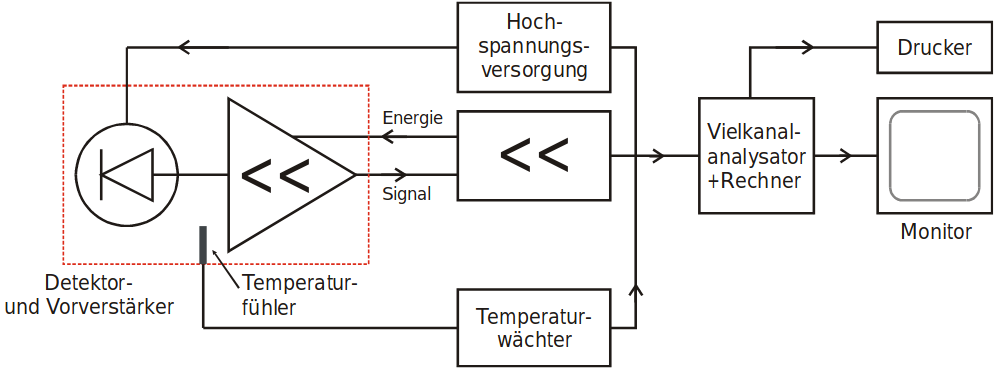
\includegraphics[scale=0.4]{Aufbau.png}
  \caption{Blockschaltbild zum Versuchsaufbau. \cite{Q1}}
  \label{abb:2}
\end{figure}



\section{Durchführung}
Zur Durchführung des Versuches wird zunächst die Gleichspannung langsam auf \SI{5}{\kilo\volt}
erhöht.
Die Probe und der Detektor befinden sich in einem mit Blei abgeschirmten Kasten,
um die Hintergrundstrahlung abzuschirmen. Außerdem ist die Bleischicht im Inneren
noch zusätzlich mit einer Kupferschicht umgeben, um gegebenenfalls strahlende
Blei-Isotope aus der Bleischicht abzuschirmen.
Nacheinander werden die jeweiligen Proben mit Hilfe eines Abstandhalters
vor dem Detektor befestigt. Die Messung wird für jede Probe ca. eine Stunde lang
durchgeführt.

\section{Auswertung}
Um die Funktionsweise des Germaniumdetektors zu untersuchen, werden nun im Folgenden die aufgenommenen
Spektren ausgewertet.

\subsection{Kalibrierung und Effizienzbestimmung des Germaniumdetektors}

Zur Kalibrierung des Germaniumdetektors wird das Spektrum eines $^{152}$Eu-Strahlers untersucht. Hierbei
werden im aufgenommenen Spektrum die Peaks detektiert und dann den im Energiespektrum von $^{152}$Eu, die der
Versuchsanleitung \cite{Q1} entnommen wurden, hervorstechenden Energiewerten zugeordnet. Das
$^{152}$Eu-Spektrum mit den detektierten Peaks ist in
Abbildung \ref{abb:Europiumspektrum} zu sehen. Die Abbildung des
Energiespektrums wurde, wie alle folgenden Plots in der Form bearbeitet, als
dass sie jeweils nur die für die Auswertung relevanten Ausschnitte aus dem
Spektrum darstellen. Weiter wurden die markierten Peaks bereits mit den, den
Kanalnummern entsprechenden Energien beschriftet. Die Berechnung der
Energiewerte erfolgte nach Gleichung \ref{eq:energie}.
Die fertige Zuordnung von Binwerten zu den Energien ist in Tabelle
\ref{tab:Kali} zu sehen.
\FloatBarrier
\begin{figure}
    \centering
    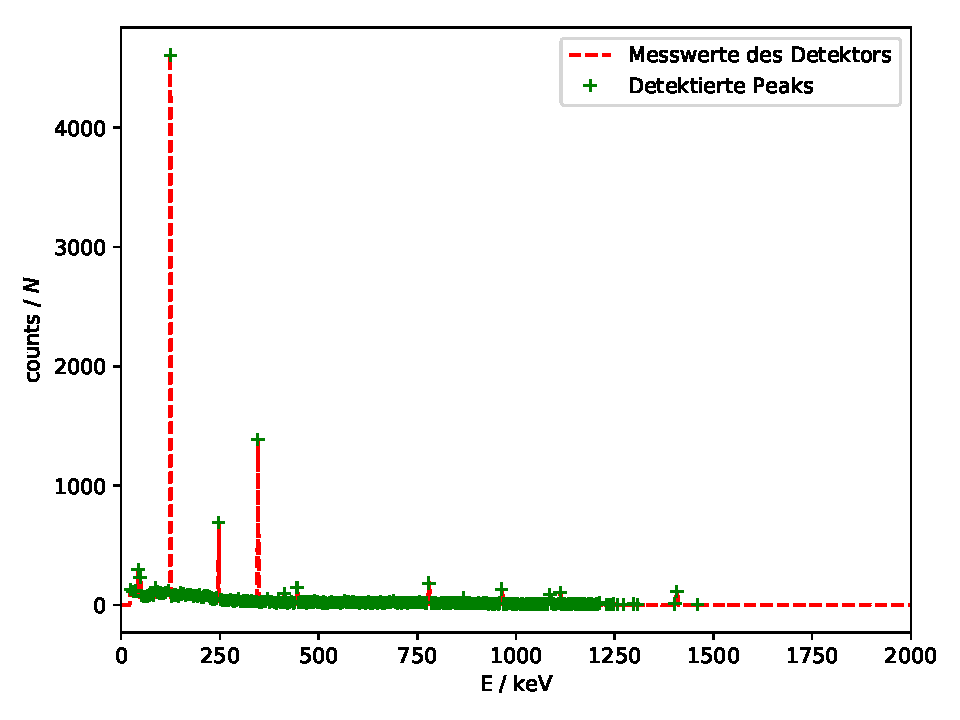
\includegraphics[scale=0.7]{Detektormesswerte.pdf}
    \caption{$^{152}$Eu-Spektrum mit detektierten Peaks.}
    \label{abb:Europiumspektrum}
\end{figure}
\FloatBarrier

\begin{table}
    \centering
    \caption{Werte zur Kalibrierung des Germaniumdetektors.}
    \label{tab:Kali}
    \begin{tabular}{ c c c c }
        \toprule
        {$\text{E}_{\gamma}$ / $\si{\kilo \electronvolt}$} & { Wahrscheinlichkeit W} & {zugeordneter Bin-Index} & {Peakhöhe}     \\
        \midrule
        121,78 &    28,6 &  309  & 4608 \\
        244,70 &     7,6 &   614  & 692 \\
        295,94 &    0,4 &   741  & 35 \\
        344,30 &     26,5 &  861  & 1388 \\
        411,12 &    2,2 &   1027 & 94 \\
        443,96 &    3,1 &   1108 & 149 \\
        678,00 &     2,0 &   1689 & 29 \\
        688,67 &    0,9 &   1715 & 35 \\
        778,90 &     12,9 &  1939 & 184 \\
        867,37 &    4,2 &   2159 & 62 \\
        964,08 &    14,6 &  2398 & 134 \\
        1005,30 &    0,6 &   2500 & 15 \\
        1085,90 &    10,2 &  2702 & 85 \\
        1112,10 &    13,6 &  2766 & 106 \\
        1299,10 &    1,6 &   3229 & 10 \\
        1408,00 &    21,0 &  3502 & 116 \\
        1457,60 &    0,5 &   3633 &   6 \\
        \bottomrule
    \end{tabular}
\end{table}
\FloatBarrier

\noindent Mittels der Zuordnung der Bin-Indizes zu den Energien kann nun eine lineare Ausgleichsrechunung der Form
\begin{align}
    E(K) = m \cdot K + n
    \label{eq:energie}
\end{align}
durchgeführt werden. Hierbei beschreibt K die Kanalnummer.
Für die Werte des linearen Fits ergibt sich dann:

\begin{align*}
    m &= \SI{0,4018 \pm 0,0007}{\kilo \electronvolt} \\
    n &= \SI{0,2(16)}{\kilo \electronvolt}
\end{align*}

\noindent Die Wertepaare aus bestehend aus dem Bin-Index und der zugeordneten Energie aus den Literaturwerten sind gemeinsam mit dem linearen Fit in Abbildung \ref{abb:linfit} zu sehen.

\FloatBarrier
\begin{figure}
    \centering
    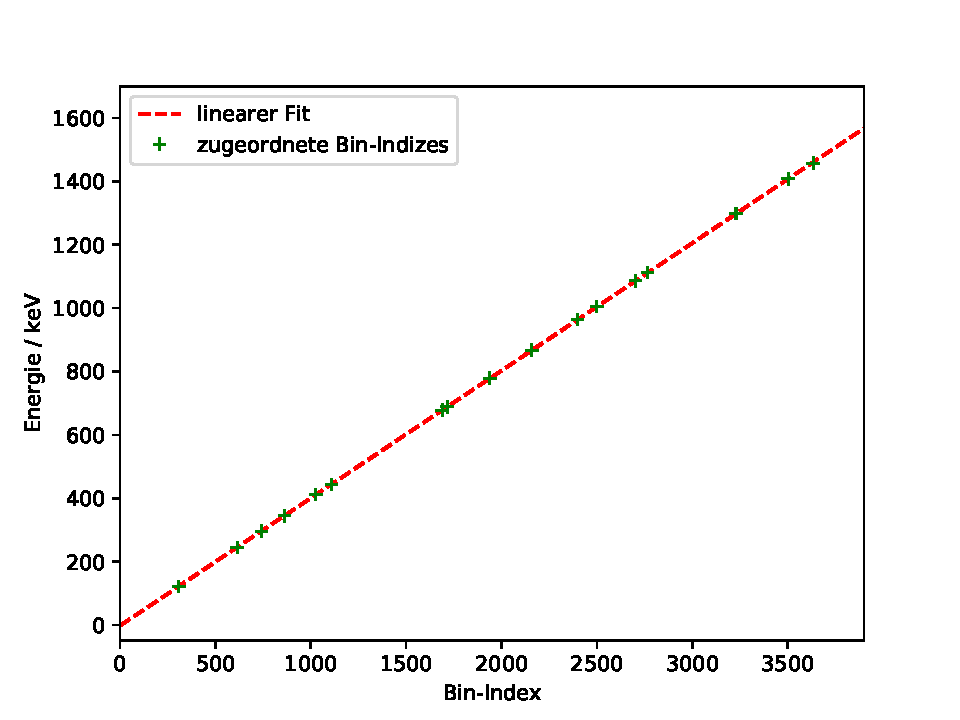
\includegraphics[scale=0.7]{Kalibrierung.pdf}
    \caption{Energiekalibrierung des Germaniumdetektors.}
    \label{abb:linfit}
\end{figure}
\FloatBarrier

\noindent Um die Effizienz des Germaniumdetektors gemäß Formel \ref{eq:effizienz} zu bestimmen, müssen
zunächst die Parameter A, Z, W und $\Omega$ ermittelt werden.
Die Aktivität A der Probe am Versuchstag, dem 07.11.2018, lässt sich mit den Angaben zur Halbwertszeit von
$^{152}$Eu ($t_{1/2}=\SI{4943(5)}{\day}$) und der Aktivität am 01.10.2000: $\text{A}_0=
\SI{4130(60)}{\becquerel}$ aus der Versuchsanleitung \cite{Q1} einfach berechnen:
\begin{align*}
    \text{A} &= \text{A}_0 \exp \left(-\frac{\ln(2) \Delta t}{t_{1/2}}\right) \\
    &= \SI{1634(24)}{\becquerel}
\end{align*}
Das Raumwinkelelement $\frac{\Omega}{4 \pi}$ berechnet sich nach Gleichung \ref{eq:Omega} mit dem Parameter
$a$ für den Abstand zwischen Quelle und Absorptionspunkt ($a=\SI{8,81}{\centi\meter}$) und $r$ für die halbe
Breite des Germaniumdetektors ($r= \SI{2,25}{\centi \meter}$). Die Wahl für $a$ ergibt sich aus der Angabe
aus der Anleitung zum Versuch \cite{Q1}, dass der wahrscheinlichste Absorptionspunkt im Germanium
$\SI{1,5}{\centi \meter}$ unter der Aluminiumhaube liegt und der Höhe des Abstandshalters zwischen Probe und
Detektor ($\SI{7,31}{\centi \meter}$).
Mit Hilfe dieser Parameter berechnet sich das Raumwinkelelement zu:
\begin{align*}
    \frac{\Omega}{4 \pi} = 0,016 \; .
\end{align*}

\noindent Die Peakinhalte zu den angegebenen Energien werden bestimmt, indem Gaußfits über jeden Peak gelegt werden. Die Gaußfits besitzen folgende Form:
\begin{equation*}
    f(K) = h \cdot \exp\left(\frac{-(K-\mu)^2}{2\sigma^2}\right) +a \;
\end{equation*}
Hierbei beschreibt $h$ die Höhe des Peaks, $\mu$ den Mittelwert, mit dem der zuvor zugeordnete Bin-Index korrigiert wird, $\sigma$ die Standardabweichung, $K$ die Kananummer und $a$ die Untergrundstrahlung.
Die Peakinhalte $Z_i$ werden dann über Integration über die Gaußkurven berechnet:
\begin{equation*}
    Z_i = \sqrt{2\pi} \cdot h_i \cdot \sigma_i
\end{equation*}
\FloatBarrier
Die sich ergebenden Parameter und Ergebnisse für die Peakinhalte $Z_i$, sowie die berechneten Effizienzen
($Q(E_i)$) sind in den Tabellen \ref{tab:effizienz1} und \ref{tab:effizienz2} zu sehen.
Anschließend wird ein nicht linearer Fit der Werte für $E_i$ und $Q(E_i)$ vorgenommen, der folgende Form
besitzt:
\begin{equation*}
    Q(E) = a \cdot \left( \frac{E}{\si{1}{\kilo \electronvolt}}\right)^{b}
\end{equation*}
Hierbei ist zu beachten, dass lediglich Energien berücksichtigt werden, die größer als $\SI{150}{\kilo
\electronvolt}$ sind.
Für die Fitparameter ergeben sich folgende Werte:
\begin{align*}
 a &= \SI{1.21(49)}{} \\
 b &= \SI{-1.10(6)}{} \; .
\end{align*}

Die Wertepaare, als auch die gefittete Potenzfunktion, sind in Abbildung \ref{abb:effizienz} zu sehen.
\FloatBarrier
\begin{table}
    \centering
    \caption{Werte zur Effizienbestimmung aus den Gaußfits}
    \label{tab:effizienz1}
    \begin{tabular}{ c c c c }
        \toprule
        {$\sigma_i$}            & {$\mu_i$}             & {$h_i$}           & {$a_{i}$}         \\
        \midrule

        1,130 \pm  0,005        & 308,800 \pm  0,005    & 4579 \pm  18      & 90 \pm  4         \\
        1,293 \pm  0,014        & 613,806 \pm  0,013    & 652 \pm  6        & 38,5 \pm  1,3     \\
        1,40 \pm  0,28          & 741,45 \pm   0,27      & 28 \pm  5         & 26,2 \pm  1,1     \\
        1,547 \pm  0,014        & 860,911 \pm  0,013    & 1349 \pm  10      & 20,1 \pm  2,6     \\
        1,80 \pm  0,08          & 1026,69 \pm  0,07     & 80.6 \pm  2,9     & 17,5 \pm  0,8     \\
        1,58 \pm  0,06          & 1108,16 \pm  0,06     & 125 \pm  4        & 15,8 \pm  1,0     \\
        1,3 \pm  0,4            & 1689,2  \pm  0,4       & 12.0 \pm  3,5     & 14,5 \pm  0,8     \\
        1,01 \pm  0,27          & 1715,07 \pm  0,26     & 19 \pm  4         & 14,6 \pm  0,9     \\
        2,58 \pm  0,06          & 1939,19 \pm  0,05     & 166.9 \pm  3,1    & 12,0 \pm  1,1     \\
        2,44 \pm  0,17          & 2158,90 \pm  0,16     & 47.7 \pm  2,7     & 13,0 \pm  1,0     \\
        3,24 \pm  0,13          & 2398,51 \pm  0,11     & 123 \pm  4        & 6,5 \pm  1,7      \\
        1,01 \pm  0,34          & 2500,23 \pm  0,33     & 9.1 \pm  2,6      & 6,1 \pm  0,5      \\
        3,18 \pm  0,14          & 2700,87 \pm  0,12     & 75.9 \pm  2,6     & 9,8 \pm  1,1      \\
        3,35 \pm  0,13          & 2766,14 \pm  0,11     & 98.5 \pm  3,0     & 5,7 \pm  1,4      \\
        0,84 \pm  0,22          & 3228,31 \pm  0,21     & 9.1 \pm  2,0      & 2,37 \pm  0,35    \\
        3,63 \pm  0,15          & 3501,10 \pm  0,12     & 103.2 \pm  3,2    & 2,4 \pm  1,6      \\
        6,2 \pm  1,6            & 3630,4 \pm  1,0       & 3.4 \pm  0,6      & 0,0 \pm  0,6      \\

        \bottomrule
    \end{tabular}
\end{table}

\FloatBarrier
\begin{table}
    \centering
    \caption{Werte zur Effizienzbestimmung aus den Gaußfits}
    \label{tab:effizienz2}
    \begin{tabular}{ c c c }
        \toprule
        {$Z_i$}             & {$E_i$ / $\si{\kilo\electronvolt}$} & {$Q(E_i)$ }               \\
        \midrule
        12970 \pm  80       & 122,1847 \pm  0,0021                & -                         \\
         2113 \pm  29       & 244,989 \pm  0,005                  & 0,284 \pm  0,006          \\
           97 \pm  25       & 296,38 \pm  0,11                    & 0,25 \pm  0,07            \\
         5230 \pm  60       & 344,481 \pm  0,005                  & 0,202 \pm  0,004          \\
          364 \pm  21       & 411,230 \pm  0,030                  & 0,169 \pm  0,010          \\
          496 \pm  24       & 444,032 \pm  0,022                  & 0,164 \pm  0,008          \\
           39 \pm  17       & 677,97 \pm  0,17                    & 0,020 \pm  0,009          \\
           49 \pm  17       & 688,39 \pm  0,11                    & 0,055 \pm  0,019          \\
         1080 \pm  32       & 778,630 \pm  0,022                  & 0,0856 \pm  0,0028        \\
          292 \pm  26       & 867,09 \pm  0,06                    & 0,071 \pm  0,007          \\
         1000 \pm  50       & 963,57 \pm  0,05                    & 0,070 \pm  0,004          \\
           23 \pm  10       & 1004,52 \pm  0,13                   & 0,039 \pm  0,017          \\
          604 \pm  34       & 1085,31 \pm  0,05                   & 0,0606 \pm  0,0035        \\
          830 \pm  40       & 1111,58 \pm  0,05                   & 0,0621 \pm  0,0032        \\
           19 \pm  6        & 1297,67 \pm  0,08                   & 0,012 \pm  0,004          \\
          940 \pm  50       & 1407,50 \pm  0,05                   & 0,0458 \pm  0,0024        \\
           53 \pm  17       & 1459,6 \pm  0,4                     & 0,108 \pm  0,035          \\
        \bottomrule
    \end{tabular}
\end{table}
\FloatBarrier
\begin{figure}
    \centering
    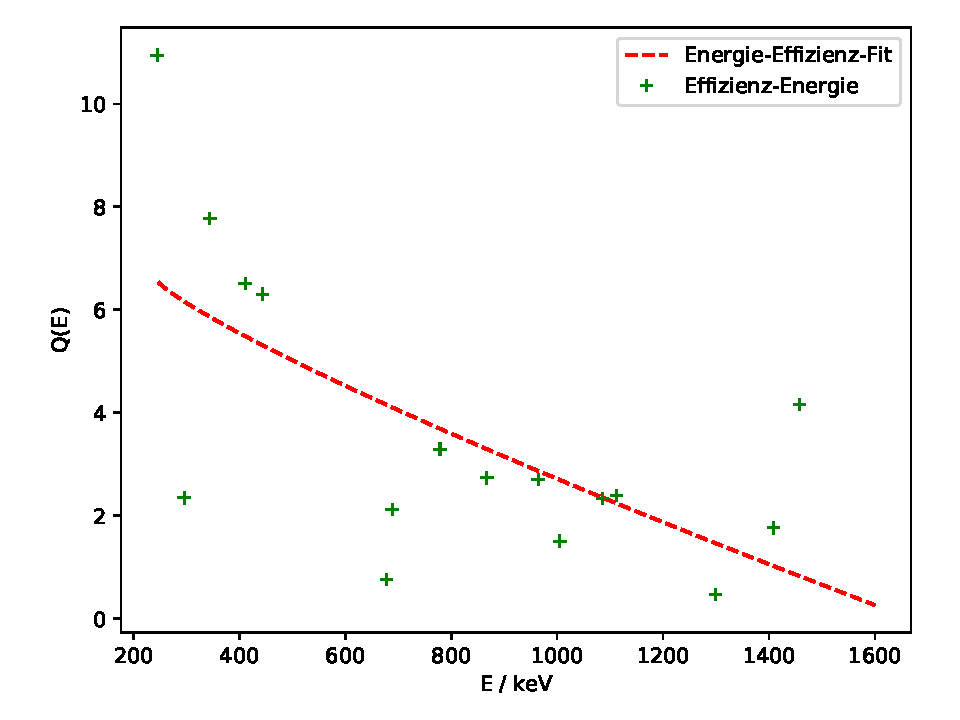
\includegraphics[scale=0.7]{effizienz.pdf}
    \caption{Effizienz des Germaniumdetektors gegen die Energie aufgetragen.}
    \label{abb:effizienz}
\end{figure}
\FloatBarrier

\subsection{Untersuchung der Halbwertsbreite des Photopeaks eines $^{137}$Cs-Strahlers}

Um die Halbwertsbreite des Photopeaks eines $^{137}$Cs-Strahlers zu untersuchen,
wird das Spektrum eines monochromatischen Gammastrahlers, das von $^{137}$Cs,
aufgenommen. Das erhaltene Spektrum ist zusammen mit den detektierten Peaks in
Abbildung \ref{abb:Cs_peaks} zu sehen. Die für die Auswertung wichtigen Peaks sind der
Photopeak, der Rückstreupeak sowie die Compton-Kante. Die erhaltenen Werte für die
Bin-Indizes sowie die zugehörigen Energiewerte sind in Tabelle \ref{tab:Cs_peaks}
dargestellt.

\FloatBarrier
\begin{figure}
    \centering
    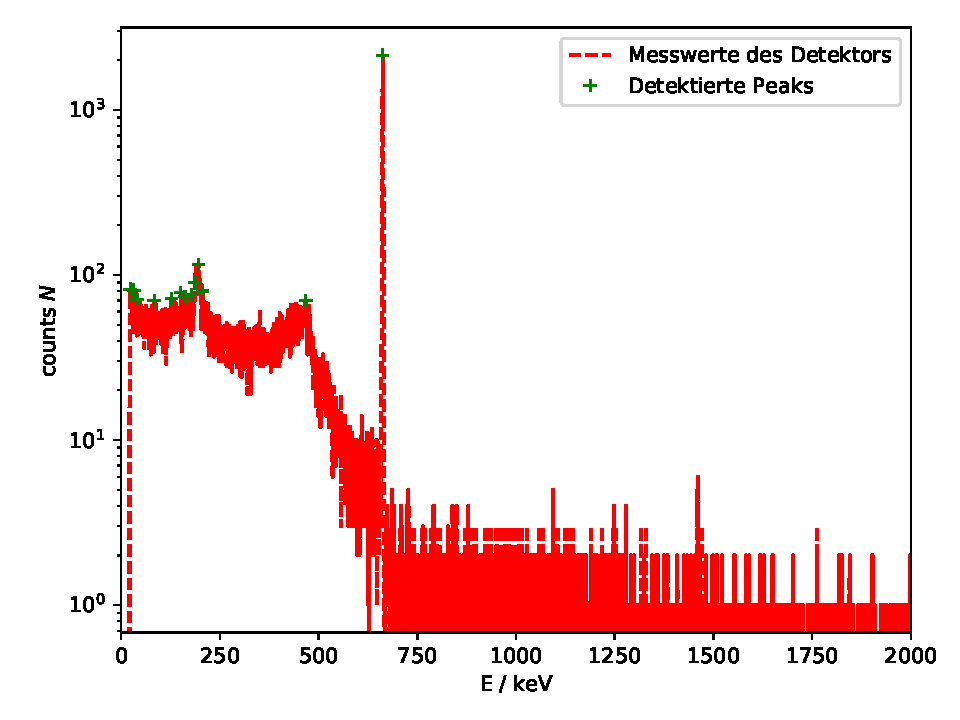
\includegraphics[scale=0.7]{Cs_fit.pdf}
    \caption{Comptonkontinuum und Photopeak des $^{137}$Cs-Strahlers.}
    \label{abb:Cs_peaks}
\end{figure}
\FloatBarrier

\begin{table}
    \centering
    \caption{Lage und Energie der charakteristischen Peaks des $^{137}$Cs-Strahlers}
    \label{tab:Cs_peaks}
    \begin{tabular}{ c c c }
        \toprule
        & {Bin-Index} & {Energie $E_i$}      \\
        \midrule
        {Rückstreupeak} & 486  & 195,44      \\
        {Compton-Kante} & 1164 & 467,87      \\
        {Photopeak}     & 1648 & 662,35      \\
        \bottomrule
    \end{tabular}
\end{table}
\FloatBarrier
Bei der Analyse der Lage der Peaks ist zu erkennen, dass die Energie des Photopeaks mit $\SI{662,35}{\kilo \electronvolt}$ sehr nah am Theoriewert ($\SI{661,59}{\kilo \electronvolt}$) liegt \ref{Q3}.
Der Theoriewert für Rückstreupeak und Compton-Kante kann wie folgt aus der Energie des Photopeaks berechnet werden:
\begin{align*}
    E_{\text{comp,theo}} &= E_\text{photo} \frac{2\epsilon}{1+2\epsilon} = \SI{477,98}{\kilo\electronvolt} \\ \Delta E_\text{comp} &= \SI{2,11}{\percent} \\
    E_{\text{rück,theo}} &= E_\text{photo} \frac{1}{1+2\epsilon} = \SI{184,38}{\kilo\electronvolt} \\
    \Delta E_\text{rück} &= \SI{6,00}{\percent}
\end{align*}
In dieser Berechnung beschreibt $\epsilon$ das Verhältnis zwischen der Energie des Photopeaks $E_\text{photo}$ zur Ruheenergie eines Elektrons: $\epsilon = \frac{E_\text{photo}}{m_e c^2}$.

\noindent Im Anschluss daran wird überprüft, ob der Photopeak Gauß-förmig ist.
Dies geschieht, indem die Flanken des Peaks mittels linearer Ausgleichsrechnung approximiert werden. Die graphische Darstellung des Vorgehens ist in Abbildung \ref{fig:Cs_photo} zu sehen.
Somit kann leicht die Halbwerts- und Zehntelwertsbreite ermittelt werden. Stehen die beiden Breiten in einem bestimmten Verhältnis zueinander, so kann davon ausgegangen werden, dass der Peak Gauß-förmig ist.
Die graphische Darstellung des Vorgehens ist in Abbildung \ref{fig:Cs_Photo} zu sehen.
Die lineare Ausgleichsrechung hat die Form $F(K) = m \cdot K + n$. Hierbei beschreibt $K$ die Kanalnummer.
Für die Parameter links (l) und rechts (r) am Peak ergeben sich folgende Werte:
\begin{align*}
    m_l &= 0,0028 \pm 0,0003 & m_r &= -0,00213 \pm 0,00018 \\
    n_l &= 1641,9 \pm 0,4    & n_r &=  1652,94 \pm 0,25
\end{align*}
Die Berechnung der Halbwerts- und Zehntelwertsbreite erfolgt mittels folgender Rechnung:
\begin{align*}
    \Delta_{h} = m_r K h + n_r - (m_l K h + n_l) \; \text{mit} \; h \in \{0,1 \; , \; 0,5\} \;
\end{align*}
Hierbei ist $K$ die Kanalnummer des Photopeaks.
Die Umrechnung des Ergebnisses in Energien, erfolgt gemäß Formel \ref{eq:energie}.
Für die Halbwerts- und Zehntelwertsbreite ergeben sich somit folgende Werte:
\begin{align*}
    \Delta_{0,5} &= \SI{2,45(23)}{\kilo \electronvolt}\\    %An Kommata denken.
    \Delta_{0,1} &= \SI{4,16(18)}{\kilo \electronvolt} \; . %An Kommata denken.
\end{align*}
Für eine Gaußverteilung gilt:
\begin{align*}
    \Delta_{0,1} &= 1,823 \cdot \Delta_{0,5} \\
                 &= \SI{4,3(4)}{\kilo \electronvolt} \; .
\end{align*}
Der mit Hilfe der Halbwertsbreite berechnete Wert für die Zehntelwertsbreite weicht
dabei lediglich um $\SI{4}{\percent}$ von dem experimentell ermittelten ab, weshalb
davon auszugehen ist, dass eine Gaußverteilung vorliegt.
Die theoretische Halbwertsbreite und somit der Wert für das theoretische Auflösungsvermögen berechnet sich gemäß Formel \ref{eq:halbwertsbreite} zu:
\FloatBarrier
\begin{align}
    \label{eq:halbwertsbreite_theo}
    \Delta E_{1/2} = \SI{1,029}{\kilo \electronvolt}
\end{align}
\FloatBarrier
Hierzu wird die zuvor ermittelte Energie des Photopeaks und die
Anregungsenergie eines Elektrons in Germanium ($\SI{2,9}{\electronvolt}$ )
verwendet.
\FloatBarrier
\begin{figure}
    \centering
    \includegraphics[scale=0.7]{Cs_photo.pdf}
    \caption{Graphische Darstellung des Gaußfits mit an die Flanken gefitteten Geraden zur Ermittlung der Halbwerts- und Zehntelwertsbreite.}
    \label{fig:Cs_photo}
\end{figure}
\FloatBarrier

\noindent Im letzten Teil des Versuchs werden die Verhältnisse der Inhalte des Comptonkontinuums und des Photopeaks und die Absorptionswahrscheinlichkeiten für Photo- und Comptoneffekt verglichen.
Die Extinktionskoeffizienten $\mu$ ergeben sich aus Abbildung \ref{abb:1}, woraus anschließend die Absorptionswahrscheinlichkeiten berechnet werden können ($p = 1-\exp(-\mu l)$). Hierbei beschreibt $l= \SI{3,9}{\centi \meter}$ die Länge des Detektors.
\begin{align*}
    \mu_{\text{comp}} &= \SI{0,38}{\per \centi \meter} \\
    p_{\text{comp}} &= \SI{77,28}{\percent}\\
    \mu_{\text{photo}} &= \SI{0,002}{\per \centi \meter} \\
    p_{\text{photo}} &= \SI{0,78}{\percent} \\
    \frac{p_{\text{comp}}}{p_{\text{photo}}} &= \SI{99,47}{}
\end{align*}
Der Inhalt des Photopeaks wird auch in diesem Teil des Versuchs ermittelt, indem er mit einem Gaußfit gefittet wird. Der Inhalt des Comptonkontinuums wird ermittelt, indem über die zugehörigen Kanalinhalte summiert wird:
\begin{align*}
    Z_{\text{comp}}  &= \SI{55000(800)}{\text{Zählungen}} \\
    Z_{\text{photo}} &= \SI{12010(100)}{\text{Zählungen}}\\
    \frac{Z_{\text{comp}}}{Z_{\text{photo}}} &= \SI{4,6(6)}{} \; .
\end{align*}
Es zeigt sich, dass der Inhalt des Photopeaks zwar kleiner ist, als der des
Comptonkontinuums, jedoch nicht in der Art, wie es der deutlich größere Absorptionskoeffizient hätte erwarten lassen.
Es kann daher davon ausgegangen werden, dass die Elektronen nicht nur einmalig Energie beim Comptoneffekt abgeben, sondern mehrfach, bevor sie dann ihre komplette Energie durch den Photoeffekt verlieren.


\subsection{Aktivität einer $^{133}$Ba-Quelle}

\noindent In diesem Teil des Versuchs wird das Spektrum eines $^{133}$Ba-
Strahlers untersucht.
Die Detektormesswerte, sowie die ermittelten Peaks der Bariumquelle sind in Abbildung \ref{abb:BaPlot} dargestellt die Messzeit betrug $\SI{3790}{\second}$.
Dafür werden die Peaks zunächst analog zum ersten Teil
des Versuchs detektiert, anschließend Gauß-gefittet und die Peakinhalte werden
ermittelt, indem über die Gaußfits integriert wird. Die zugeordneten Bin-
Indizes, sowie die gemäß Formel \ref{eq:energie} aus den Kanalnummern
berechneten Energien, sind in Tabelle \ref{tab:BaTab} dargestellt.
\FloatBarrier
\begin{figure}
    \centering
    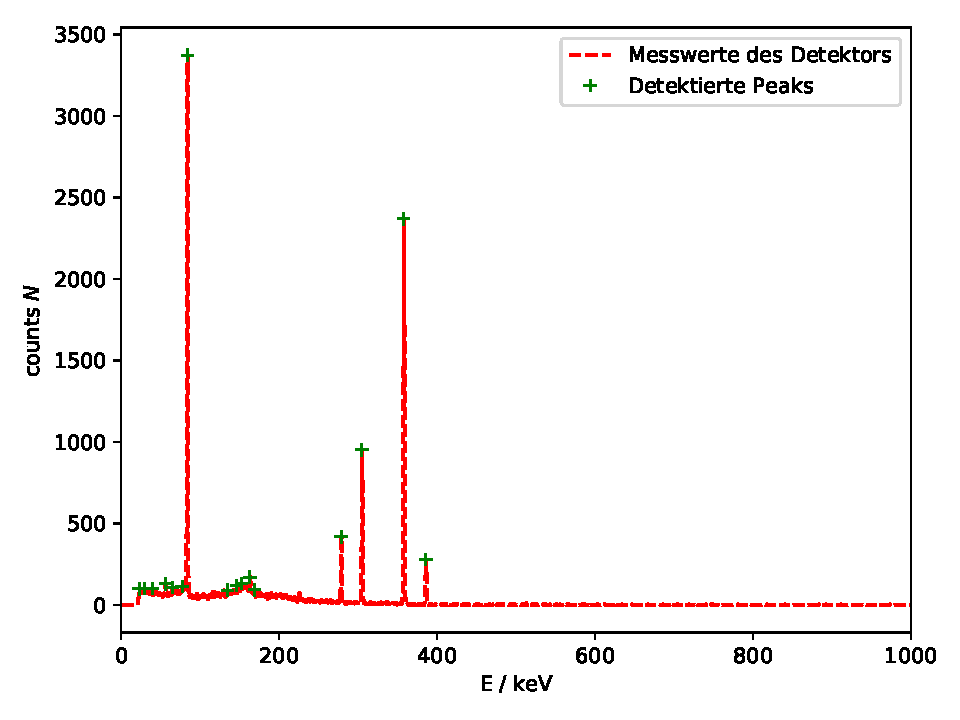
\includegraphics[scale=0.7]{Ba_plot_peaks.pdf}
    \caption{Spektrum mit detektierten Peaks einer $^{133}$Ba-Quelle.}
    \label{abb:BaPlot}
\end{figure}
\FloatBarrier

\begin{table}
    \centering
    \caption{Zugeordnete Peaks und Bins einer $^{133}$Ba-Quelle. }
    \label{tab:BaTab}
    \begin{tabular}{cccc}
        \toprule
        {E / keV} & { W } & zugeordneter Bin-Index & berechnete Energie \\
        \midrule
        53,16   &   2,2     &   139,0  &    55,86\pm0,07      \\
        810    &   34,1     &   208,0  &    83,575\pm0,008    \\
        160,61  &   0,6     &   405,0  &    163,00\pm0,09     \\
        276,40  &   7,2     &   693,0  &    278,466 \pm 0,078  \\
        302,85  &   18,3    &   758,0  &    304,7824\pm0,0026 \\
        356,02  &   62,1    &   890,0  &    357,8077\pm0,0030 \\
        383,85  &   8,9     &   960,0  &    385,616\pm0,010   \\
        \bottomrule
    \end{tabular}
\end{table}
\FloatBarrier

\noindent Mit Hilfe der Formel für die Ermittlung der Effizienz \ref{eq:effizienz}, kann so ein Wert für die Aktivität der Bariumquelle ermittelt werden. Hierbei ist darauf zu achten, dass nur Werte mit einer Energie $E_i$ größer als $\SI{150}{\kilo \electronvolt}$ verwendet werden, da nur für diese Werte die Effizienz bestimmt werden kann.
Die Werte, die sich für die Bin-Indizes, die Standardabweichung, die Höhe der Peaks, die Peakinhalte, die Energie sowie die Aktivität der Quelle ergeben, sind in den Tabellen \ref{tab:BaAkt} \ref{tab:BaAkt2} dargestellt.
\FloatBarrier
\begin{table}
    \centering
    \caption{Ergebnisse zur Bestimmung der Aktivität der $^{133}$Ba-Quelle.}
    \label{tab:BaAkt}
    \begin{tabular}{ c c c }
        \toprule
        {$\sigma_{\text{ba}}$} & {$h_i$} &  {$a_i$}                     \\
        \midrule
        0,85 \pm 0,19     & 64 \pm 12              &     71,6 \pm 1,5   \\
        1,081 \pm 0,020   & 3490\pm 50             &     84 \pm 8       \\
        0,79 \pm 0,23     & 84 \pm 21              &     89,3 \pm 2,6   \\
        1,367 \pm 0,017   & 413 \pm 4              &     16,6 \pm 0,8   \\
        1,384 \pm 0,007   & 930 \pm 4              &     12,9 \pm 0,7   \\
        1,513 \pm 0,008   & 2403 \pm 10            &     8,0 \pm 1,9    \\
        1,657 \pm 0,027   & 286 \pm 4              &     2,9 \pm 0,8    \\
        \bottomrule
    \end{tabular}
\end{table}
\FloatBarrier
\begin{table}
    \centering
    \caption{Ergebnisse zur Bestimmung der Aktivität der $^{133}$Ba-Quelle.}
    \label{tab:BaAkt2}
    \begin{tabular}{ c c c }
        \toprule
        {Bin-Index} & {Peakinhalt $Z_i$} & {Aktivität $A_i$ / $\si{\kilo \becquerel}$} \\
        \midrule
        138,62 \pm 0,17    & 130 \pm 40         & - \\
        207,604 \pm 0,017  & 9480 \pm 200       & - \\
        405,26 \pm 0,23    & 190 \pm 70         & 1,024\pm0,388\\
        692,542 \pm 0,017  & 1417 \pm 23        & 1,321\pm0,021 \\
        758,119 \pm 0,006  & 3227 \pm 18        & 1,307\pm0,008 \\
        890,082 \pm 0,007  & 9120 \pm 50        & 1,300\pm0,009 \\
        959,288 \pm 0,023  & 1187 \pm 22        & 1,283\pm0,027 \\
        \bottomrule
    \end{tabular}
\end{table}
\FloatBarrier
Die erhaltenen Werte für die Aktivität werden anschließend gemittelt, wodurch sich folgender Wert für die Aktivität der $^{133}$Ba-Quelle ergibt:
\begin{align*}
    A_\text{Ba} = \SI{1,25(9)}{\kilo \becquerel}
\end{align*}
\FloatBarrier


\subsection{Aktive Nuklide eines unbekannten Strahlers}
Im finalen Teil des Versuchs wird eine unbekannte Substanz im Germaniumdetektor analysiert. Das Spektrum, sowie die detektierten Peaks sind in Abbildung \ref{abb:unbekannt} zu sehen. Die Position sowie die Höhe und zugehörige Energie sind in Tabelle \ref{tab:unbekannt} zu sehen.
\FloatBarrier
\begin{figure}
    \centering
    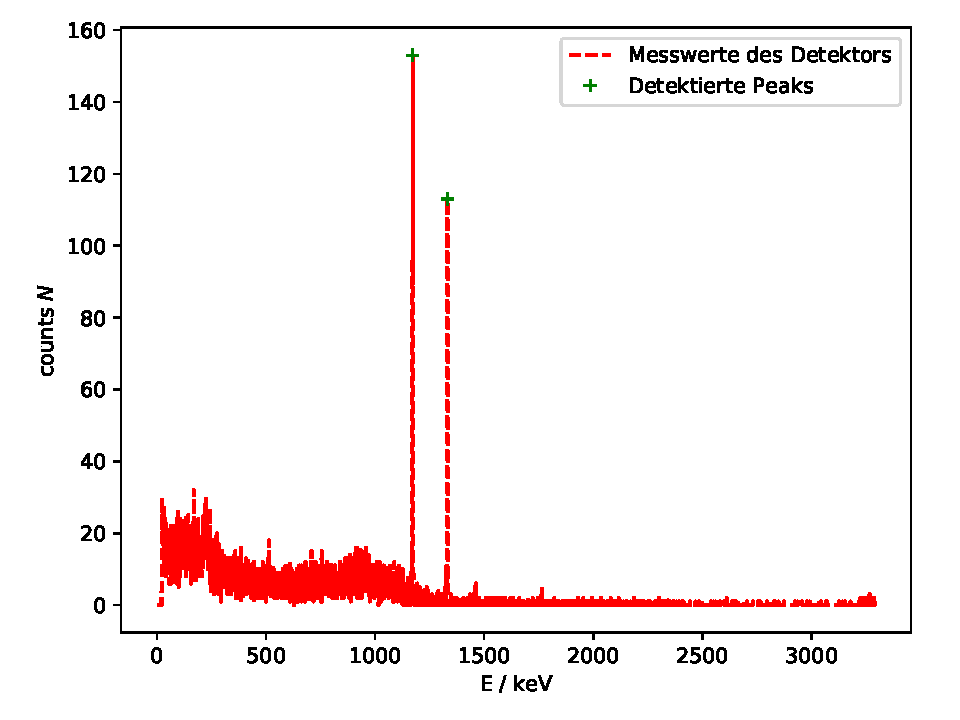
\includegraphics[scale=0.7]{unbekannterStrahler.pdf}
    \caption{Emissionsspektrum mit detektierten Peaks des unbekannten Strahlers.}
    \label{abb:unbekannt}
\end{figure}
\FloatBarrier
\begin{table}
    \centering
    \caption{Detektierte Peaks und zugeordnete Energie des unbekannten Strahlers.}
    \label{tab:unbekannt}
    \begin{tabular}{ c c c }
    \toprule
    {Bin-Index} & {counts } & {Energie $E_i$ / $\si{\kilo\electronvolt}$}\\
    \midrule
    2918 & 153.0 & 1172.66       \\
    3313 & 113.0 & 1331.38       \\
    \bottomrule
    \end{tabular}
\end{table}
\FloatBarrier

\noindent Die Energien der ermittelten Peaks werden anschließend mit Literaturwerten für verschiedene Gammastrahler verglichen. Wichtigstes Merkmal des unbekannten Gammastrahlers sind in diesem Spektrum die einzigen zwei deutlich hervorstechenden Peaks bei $\SI{1172,66}{\kilo \electronvolt}$ und $\SI{1331,38}{\kilo \electronvolt}$. Diese beiden Peaks passen sehr gut zu den beiden Peaks des $^{60}$Co, die laut Literaturangaben \cite{Q4} $\SI{1,173}{\mega \electronvolt}$ und $\SI{1,332}{\mega \electronvolt}$ betragen sollen.

\section{Diskussion}
Im ersten Teil des Versuchs konnte der lineare Zusammenhang zwischen Bin-Index
und der Energie gut sichtbar gemacht werden.
Die große Abweichung im Fitparameter $n$ ist eventuell dadurch erklärbar, dass
sich die niedrigen Peaks mit wenigen Counts nicht gut über Gaußfits
approximieren lassen. Außerdem werden für die Erstellung des Fits die
unkorrigierten Channelnummern verwendet.

\noindent Die hohe Präzision des Germaniumdetektors ist an der sehr geringen
Abweichung von $\SI{0,1}{\percent}$ des detektierten Wertes für die Energie des
Photopeaks vom Literaturwert \cite{Q3} erkennbar. Ebenso spricht die Abweichung
der Compton-Kante mit lediglich zwei Prozent vom Theoriewert für die hohe
Präzision des Detektors. Die etwas höhere Abweichung des Theoriewertes für den
Rückstreupeak ist dadurch zu erklären, dass der theoretische Wert nur als eine
Näherung zu betrachten ist und das Ablesen des Peaks eine gewisse Ungenauigeit
birgt.
Die Emissionslinien des unbekannten Strahlers konnten deutlich dargestellt und
mit den Theoriewerten verglichen werden. Es ist leicht zu erkennen, dass das
detektierte Spektrum dem von $^{60}Co$ entspricht. Die Energien weisen eine
sehr geringe Abweichung von $\SI{0,05}{\percent}$ für den detektierten Peak mit
$\SI{1331,38}{\kilo \electronvolt}$ und $\SI{0,03}{\percent}$ für den Peak mit
$\SI{1172,66}{\kilo \electronvolt}$. Dies spricht abermals für das sehr gute
Auflösungsvermögen des Germaniumdetektors, worauf auch die sehr geringe Halbwertsbreite von $\SI{2,45(23)}{\kilo \electronvolt}$ schon hinweist.

\noindent Bei der Ermittlung der theoretischen Halbwertsbreite
(siehe Gleichung \ref{eq:halbwertsbreite_theo} ) fällt auf, dass diese deutlich kleiner ist, als
der experimentell ermittelte Wert. Dies ist durch die immer noch vorhandene
Untergrundstrahlung zu erklären, die von dem im Versuch verwendeten
Germaniumdetektor nicht abgeschirmt werden kann.


\printbibliography
